
	%% setup reference database.
	\bibliography*{20131020oldnotes}
	\bibliographystyle*{bibstyle}     %% setup reference style.
	%% Section title
\section{以前的笔记备份}
\section*{写在前面的话}
无数人在我的面前说科研需要记录,无数的人的经验都表明科研需要积累,需要反复地琢磨,每当前辈们再谈她们的科研
时,都会津津乐道地谈一件之前没有发现的诀窍,忽然有一天灵感来了,注意是灵感来了,一下子就豁然开朗,成就了自
己的事业,这是我所能听说的,看见的,还有我听不见看不见的,需要自己来体会。科研是团队的事情,但是每一个科研
人员都是参与其中的,这种参与感不会是看不见摸不着,但是随着时间的流逝,这种感觉会越来越淡。于是而我们需要记
录需要记录这一路的艰辛,记录繁复的科研流程,在科研的旅行中记录,当时光流逝,是怎样的心路历程。最好当我抓耳
挠腮不知道该怎么办的时候,翻阅这样的笔记的时候,灵感能像苹果一样砸到我的脑门上,哈哈!

\newpage
\section{非线性快速多极边界元算法的一些实现}
边界辐射是一种非线性现象,需要进行非线性迭代,这次去暑期班的时候,老师讲了一种Matrix free Newton迭代方法,不需要求解雅克比矩阵,而且只依赖于矩阵向量乘法,这种方法是这样的:

\subsection{无矩阵牛顿方法}
首先,Newton方法是要计算出雅克比矩阵$J$,然后计算迭代增量$\Delta x = J^{-1}F(x_k)$,并且$J$矩阵未必是满矩阵,
这是由于PDE的性质,只与周围的点相关,与距离比较远的点无关。因此求迭代增量的时候就可以用如下的方法。
%\begin{figure}[htbp]
	\begin{center}
		\includegraphics[width=0.8\textwidth]{pics/Matrixfreenewtonmethod.eps}
	\end{center}
	%\caption{无矩阵牛顿迭代方法}
	%\label{fig:newton}
%\end{figure}

采用上面的方法来构造非线性迭代求解。

\subsection{快速多极算法的非线性迭代方法选择}

快速多极算法本质上就是通过对边界积分方程的核函数进行截断展开,与只依赖于矩阵向量乘法的线性方程组求解器结合,设计了一套算法来加速求解矩阵向量乘法的过程,通常采用的是GMRES算法,但是从文献中看到的另一个观点就是
\begin{quote}
	\kaishu
如果矩阵向量乘法的代价是昂贵的,(比如矩阵是稠密的或者不可能加快矩阵向量乘法)那么GMRES是一个比较合适的算法,因为他相对其他算法来说需要最少次数的矩阵向量乘法来达到给定的误差限。

如果矩阵向量乘法代价不是那么昂贵,又或者使用(full)GMRES方法没有在足够的存储空间时,采用BiCG相关的一些方法是比较好的选择,而且更倾向与选择使用QMR方法。
	
\end{quote}

这样看来使用GMRES来配合快速多极算法并不是很合适,因为矩阵向量乘法在快速多极算法里面不是很昂贵,毕竟快速多
极算法本身就是来降低矩阵向量乘法的计算量和存储量的,而且使用GMRES比BICG,QMR方法更加占用内存。

\section{计算均匀化方法}

\subsection{计算均匀化方法的源起}
计算均匀化方法是一种多尺度分析方法\cite{ozdemir2008computational,Geers20102175},他可以看作是一种局部-全局分析方法,
宏观预测不是基于材料的完整模型,而是依赖于材料点处微观结构的详尽模型。

\subsection{换热问题的计算均匀化}
\subsubsection{宏观方程}
宏观方程描述与时间相关的换热问题,他可以表示材料温度随时间变化的过程。
\begin{equation}
	(\rho c_v)_M \dot{\theta}_M + \nabla_M \cdot \mathbf{q}_M = 0.
	\label{eq:macro}
\end{equation}
宏观的热存储项$(\rho c_v)_M$可以由下式得到,
\begin{equation}
	(\rho c_v)_M = \frac{1}{V}\int_V (\rho c_v)_m d\,V
\end{equation}
\begin{remark}	
	注意到宏观方程\eqref{eq:macro}里面的后一项是宏观的热流密度,可以从微观的问题得到。
\end{remark}

\subsubsection{微观方程}
由于微观结构的尺寸,在这个算法中微观方程被考虑为一个稳态的问题,即微观问题在代表性单元(RVE)
上满足如下的方程,
\begin{equation}
	\nabla_m \cdot \mathbf{q}_m(\mathbf{x}) = 0
\end{equation}
通常情形下,代表性单元是一个正方形区域,如图\ref{fig:rve}所示,
\begin{figure}[htbp]
	\begin{center}
		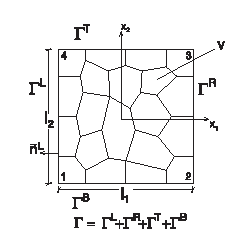
\includegraphics[width=0.3\textwidth]{pics/RVE.eps}
	\end{center}
	\caption{代表性单元}
	\label{fig:rve}
\end{figure}

\subsubsection{宏观到微观的转换}
微观温度可以表示为宏观温度的一个扰动,即可以表示为:
\begin{equation}
	\theta_m(\mathbf{x}) = \theta_m^k + \nabla_M \theta_M \cdot (\mathbf{x}-\mathbf{x}^k) + \theta_f,
	\label{eq:mac2mic}
\end{equation}
其中$\theta_m^k$表示的是RVE上任意一个参考点处$\mathbf(x)^k$的温度,不失一般性可以选取1号角点,$\theta_f$表示
的是扰动的余项利用\eqref{eq:mac2mic}可以得到微观温度梯度的体积平均为
\begin{equation}
	\frac{1}{V}\int_V \nabla_m \theta_m dV =\nabla_M\theta_M +\frac{1}{V}\int_V \theta_f \mathbf{n}d\Gamma,
	\label{eq:micavg}
\end{equation}
式\eqref{eq:micavg}中的最后一项是通过分部积分(Gauss散度定理)得到的。

式\eqref{eq:micavg}中$\nabla_M \theta_M$ 表示的是通过边界进入代表性单元的量宏观热流。尺度联合条件要求宏观温度梯度等于微观温度梯度的体积平均,即满足
\begin{equation}
	\frac{1}{V}\int_V \nabla_m \theta_m dV =\nabla_M\theta_M,	
	\label{eq:relation1}
\end{equation}
这就导致了如下的条件必须满足,
\begin{equation}
	\int_{\Gamma} \theta_f \mathbf{n}d\Gamma = 0.
	\label{eq:condrve}
\end{equation}
这个条件可以由选取RVE的边界条件来满足,即后面所讲的微观边界条件的周期性边界条件等。

\subsubsection{微观RVE的边界条件}
式\eqref{eq:condrve}可以写为
\begin{equation}
	\int_{\Gamma^L}\{\theta_f^L-\theta_f^R\}\mathbf{n}^Ld\Gamma + \int_{\Gamma^L}\{\theta_f^B-\theta_f^T\}\mathbf{n}^Bd\Gamma = 0,
\end{equation}
令$\{\theta_f^L-\theta_f^R\}=0$ 和$\{\theta_f^B-\theta_f^T\}$,并利用\eqref{eq:mac2mic}就可以得到如下的边界条件,
\begin{equation}
	\text{(周期性边界条件)}
	\begin{cases}
		\theta_m^R -\theta_m^L = \nabla_M \theta_M \cdot (\mathbf{x}^R - \mathbf{x}^L), \\
		\theta_m^T -\theta_m^B = \nabla_M \theta_M \cdot (\mathbf{x}^T - \mathbf{x}^B),
	\end{cases}
\end{equation}
定义$q_{m_n}^{(L,R,T,B)} = \mathbf{q}_m^{(L,R,T,B)} \cdot \mathbf{n}^{(L,R,T,B)}$,
则周期反法向热流边界条件为
\begin{equation}
	\text{(反周期边界条件)}
	\begin{cases}
		q_{m_n}^L &= - q_{m_n}^R, \\
		q_{m_n}^T &= - q_{m_n}^B.
	\end{cases}
\end{equation}
	

\subsubsection{微观到宏观的尺度关联}
由热力学第二定律,得到了Fourier不等式,
\begin{equation}
	-\frac{1}{\theta}\nabla\theta\cdot\mathbf{q}\geqslant 0
\end{equation}
这表示由热传导引起的熵变,参考文献\cite{ostoja2002towards},忽略掉分母上的温度,令宏观和微观层面上的熵的变化量相同,就得到
\begin{equation}
	\frac{1}{V} \int_V \nabla_m \theta_m \cdot \mathbf{q}_m \, dV = \nabla_M\theta_M\mathbf{q}_M,
	\label{eq:entropy}
\end{equation}
式\eqref{eq:entropy}表明由于热传导引起的熵的变化是保持不变的。

式\eqref{eq:entropy}的左边可以写为
\begin{equation}
	\frac{1}{V} \int_V \nabla_m \theta_m \cdot \mathbf{q}_m \, dV = \frac{1}{V}\int_{\Gamma}\theta_m q_{m_n} d\Gamma
	\label{eq:entropy2}
\end{equation}
式\eqref{eq:entropy2}中使用了Gauss定理以及如下的关系式,
\begin{eqnarray*}
	\nabla_m \cdot (\theta_m\mathbf{q}_m) &=& \nabla_m\theta_m\cdot \mathbf{q}_m + \theta_m \cdot \color{blue}{\nabla_m \cdot \mathbf{q}_m} ,\\
	\nabla_m \cdot \mathbf{q}_m &=& 0 ,\\
	q_{m_n} &=& \mathbf{q}_m \cdot \mathbf{\hat{n}}.
\end{eqnarray*}

微观热流场的体积平均可以写为
\begin{equation}
	\frac{1}{V} \int_{V} \mathbf{q}_m dV = \frac{1}{V} \int_{\Gamma} \mathbf{x}q_{m_n} d \Gamma,
	\label{eq:microheatflux}
\end{equation}
式~\eqref{eq:microheatflux}利用了Gauss定理以及如下的关系,
\begin{eqnarray*}
	\nabla_m \cdot (\mathbf{x}_m \mathbf{q}_m) &=& \nabla_m \mathbf{x}_m \cdot \mathbf{q}_m + \mathbf{x}_m (\nabla \cdot \mathbf{q}_m) = \mathbf{q}_m, \\
	\nabla_m \cdot \mathbf{x} &=&  \mathbf{I}.
\end{eqnarray*}

进一步利用周期性温度边界条件和反周期性热流边界条件,得到
\begin{equation}
	\begin{split}
		\frac{1}{V}\int_{\Gamma} \theta_m q_{m_n} d \Gamma &= \frac{1}{V} \nabla_M \theta_M \cdot \int_{\Gamma^{L}}(\mathbf{x}_L - \mathbf{x}_R) \mathbf{q}_m \cdot \mathbf{n}^L d \Gamma + \int_{\Gamma^{L}}(\mathbf{x}_B - \mathbf{x}_T) \mathbf{q}_m \cdot \mathbf{n}^B d \Gamma \\
		& = \nabla_M\theta_M \cdot \frac{1}{V}\int_{\Gamma}\mathbf{x}q_{m_n}d\Gamma = \nabla_M\theta_M \cdot \frac{1}{V}\int_{V}\mathbf{q}_m dV. 
	\end{split}
	\label{eq:han2}
\end{equation}
比较\eqref{eq:entropy},\eqref{eq:entropy2}和\eqref{eq:han2}就可以知道下式成立,
\begin{equation}
	\frac{1}{V} \int_{V}\mathbf{q}_m dV = \mathbf{q}_M.
	\label{eq:hflux}
\end{equation}
\begin{remark}
	式\eqref{eq:hflux}的推导过程表明在周期性温度边界条件下,RVE热流的体积平均就是宏观热流。
\end{remark}


\subsection{数值求解流程}
由上面的分析可以知道计算均匀化方法求解多尺度热传导问题归结为求解两个问题
一个是微观问题,也就是微观的RVE上的稳态问题。
\begin{equation}
	\text{\color{blue}{(微观问题(RVE))}}
	\begin{cases}
	\nabla_m \cdot \mathbf{q}_m(\mathbf{x}) = 0 \\
\text{(周期性边界条件)}
	\begin{cases}
		\theta_m^R -\theta_m^L = \nabla_M \theta_M \cdot (\mathbf{x}^R - \mathbf{x}^L) \\
		\theta_m^T -\theta_m^B = \nabla_M \theta_M \cdot (\mathbf{x}^T - \mathbf{x}^B)
	\end{cases}
	\end{cases}
	\label{eq:microeq}
\end{equation}

\begin{equation}
	\text{\color{blue}{(宏观问题)}}
	\begin{cases}
		(\rho c_v)_M \dot{\theta}_M + \nabla_M \cdot \mathbf{q}_M = 0.	\\
		\text{Macro B.C. (boundary conditions).} \\
		\text{Macro I.C.  (initial conditions).}
	\end{cases}
	\label{eq:macrosys}
\end{equation}

\begin{remark}
	由微观问题可以看到,该问题的求解需要知道$\nabla_M \theta_M$才能得到边界条件,然后才能对问题\eqref{eq:microeq}求解,而且仅仅有周期性边界条件可能得不到微观问题的唯一解(?)。
\end{remark}

宏观尺度和微观之间的量之间的关系有
\begin{eqnarray*}
	\frac{1}{V}\int_V \nabla_m \theta_m dV &=& \nabla_M\theta_M, \\
	\frac{1}{V} \int_V \nabla_m \theta_m \cdot \mathbf{q}_m \, dV &=&  \nabla_M\theta_M\mathbf{q}_M, \\
	\frac{1}{V} \int_V  \mathbf{q}_m \, dV &=&  \mathbf{q}_M.
\end{eqnarray*}
即式\eqref{eq:relation1},式\eqref{eq:entropy}和式\eqref{eq:hflux}。

\begin{remark}
	上述几个关系确定了微观尺度量到宏观尺度量之间的关系,微观问题的求解需要宏观的温度梯度来构造边界条件,而宏观问题需要计算与材料相关的宏观热流和宏观比热容宏观热传导系数等参数,而这些量可以从RVE问题的计算中得到。
\end{remark}
\subsubsection{微观问题的求解——周期性边界条件的施加}
\subsubsection{宏观问题的求解}
\subsection{宏观导热系数和宏观热流的计算}

\begin{think}
	如何用数学的观点把这个过程呈现出来?因为这个问题涉及微观到宏观的迭代,如何刻画这个迭代过程的收敛性?
\end{think}

\begin{think}
	这一套算法是利用RVE上的微观量的体积平均来做的,宏观方程中只要取积分点处的宏观量,也就是说是积分点处的微观量的体积平均,
	但是这样的方法中,\color{red}{宏观网格与RVE的选取有没关联},毕竟这个是一个嵌套的求解过程也就是所谓的$FE^2$过程,微观的体积平均能不能作为宏观分析的量?
\end{think}

\section{边界热辐射耦合求解的迭代求解策略}
\subsection{半耦合方法}
边界热辐射方程和热传导方程的耦合问题共有两个积分方程,给定迭代初始温度值,求解边界热辐射方程,就得到了热传导方程的边界条件,在求解热传导方程,得到新的温度值,依次迭代求解,直到收敛。
\subsection{全耦合方法}

对于边界积分方程的边界元离散,特别地针对热传导方程,其未知量不是离散点的温度就是边界点上的热流密度,二者只能
知道其一,这通常是边界条件给定的,通过求解相应的方程来求解离散点对应的另一个变量,然后通过边界积分方程恢复区
域内的变量值。


采用迭代法来求解方程的话,假设离散系统有$2N$个离散点,有关于未知量的边界积分离散方程,共$N$个,以及边界条件
共$N$个,采用迭代方法的话,设有$2N$个未知量,给定初值,就可以求解方程。

由于该方程是一个非线性方程,需要采用非线性迭代,采用前面描述过的无矩阵Newton方法,可以直接对该方程求解,称这
种方法为\textbf{全耦合方法}.

但是考虑到方程组的性质与未知变量的排序有关,因此需要考虑迭代算法的预处理,可以用区域分解方法来对这样的方程进
行处理。

\subsection{快速多极算法的并行版本}
这个方程的并行处理需要对矩阵预处理,这是一个思路,另外一个思路就是区域分解的思路。

\section{并行机架构}
\subsection{名词解释}
{胖节点}: 用于大内存串行任务,它就适用于对内存、处理性能要求高的计算任务,也就是所说的多路服务器。


\section{GMRES求解算法}
\subsection{GMRES算法过程}
GMRES算法是求解非对称线性方程组的常用算法,该算法如下所示:
\begin{algorithm}
	\caption{GMRES algorithm for solving linear systems $Ax=b$ with arbitrary (nonsigular) square matrice A}
	\begin{algorithmic}
		\STATE Let $\mathbf{q}_1 = \mathbf{b}/\|\mathbf{b}\|$ 
		\FOR{ $n = 1,2,\cdots$}
		\STATE Perform step $n$ of Arnoldi iteration;
		\STATE Find $y$ that minimizes $ \| \hat{H}_n y - \|b\|e_1\|_2$;
		\STATE Set $x_n=Q_n y$.
		\ENDFOR
	\end{algorithmic}
\end{algorithm}
\begin{remark}
	GMRES 算法的计算量依赖于最小二乘算法求解$y$和Arnoldi迭代过程。并且该算法的时间复杂度是$O(m^2)$.
\end{remark}
\subsection{Arnoldi迭代过程}
\begin{algorithm}
	\caption{Arnoldi iteration}
	\begin{algorithmic}
		\STATE Let $\mathbf{b}$ be an arbitrary initial vector
		\STATE $\mathit{\mathbf{q}}_1 = \mathbf{b}/\|\mathbf{b}\|_2$
		\FOR {$n = 1, 2, 3, . . .$}
		\STATE $v = Aq_n$
		\FOR {$j = 1 : n$}
		\STATE $h_{jn} = q^*_j v$
		\STATE $v = v − h_{jn}q_j$
		\ENDFOR
		\STATE $h_{n+1n} = \|v\|_2 $
		\STATE $q_{n+1} = v/h_{n+1,n}$
		\ENDFOR
	\end{algorithmic}
\end{algorithm}
\begin{remark}
	Arnoldi迭代过程计算量最大的操作是矩阵向量乘法$Aq_n$,并且该算法中的矩阵向量乘法的结果,并不关心矩阵$A$是如何存储以及矩阵向量乘法是如何实现的。
\end{remark}

\section{求解边界热辐射问题的有限元方法和边界元方法的对比}

\subsection{有限元方法的劣势}
以蜂窝结构为例,由于网格形状的限制,采用有限元方法,对于蜂窝结构的薄壁进行较细密的网格划分,这就对增加了该问
题求解的计算量。
\subsection{采用边界元方法的原因}
采用边界元方法的出发点之一就是由于边界元方法的网格单元在二维情形下是线单元,三维情形下是面单元,对该问题的薄
壁进行形状契合的体单元划分,并且采用快速多极算法对采用边界元方法求解该方程可以加速求解,因此快速多极边界元方
法对该类问题的求解有着潜在的优势。
\begin{remark}
	对于孔洞材料的热辐射问题,采用边界元方法得到的矩阵可能是一个块加边对角矩阵,可以利用这个特性来构造一个快速
	求解算法。
\end{remark}
\section{热辐射热传导耦合边界元方法的奇异积分处理}
采用边界元方法的主要的问题有最后要求解线性方程是非对称满阵,需要计算奇异积分等,非对称满阵的问题可以由快速多
极算法来实现,奇异积分的问题也可以通过多极展开来处理,或者采用传统的方法,也许可以采用河海大学陈文教授的奇异
边界方法结合多极展开来对奇异积分进行处理。

\subsection{传统的边界元奇异积分处理}
Cauchy型奇异积分的处理,Harmand奇异积分的处理,高效伟文章中的奇异积分的处理方法。
\subsection{奇异边界方法}
查一下陈文的文章。
\subsection{快速多极边界元中奇异积分的处理方法}
需要查文献了。

\begin{think}
	我想做的一件事情就是将奇异边界方法和快速多极方法结合起来做一个很好的方法。
\end{think}
\section{孔洞材料边界元离散建模}
采用快速多极算法的孔洞材料边界元方法需要对网格单元进行树结构划分,\figref{fig:porous0_4686}就是一个自适应树结构的例子。
\begin{figure}[htbp]
	\begin{center}
		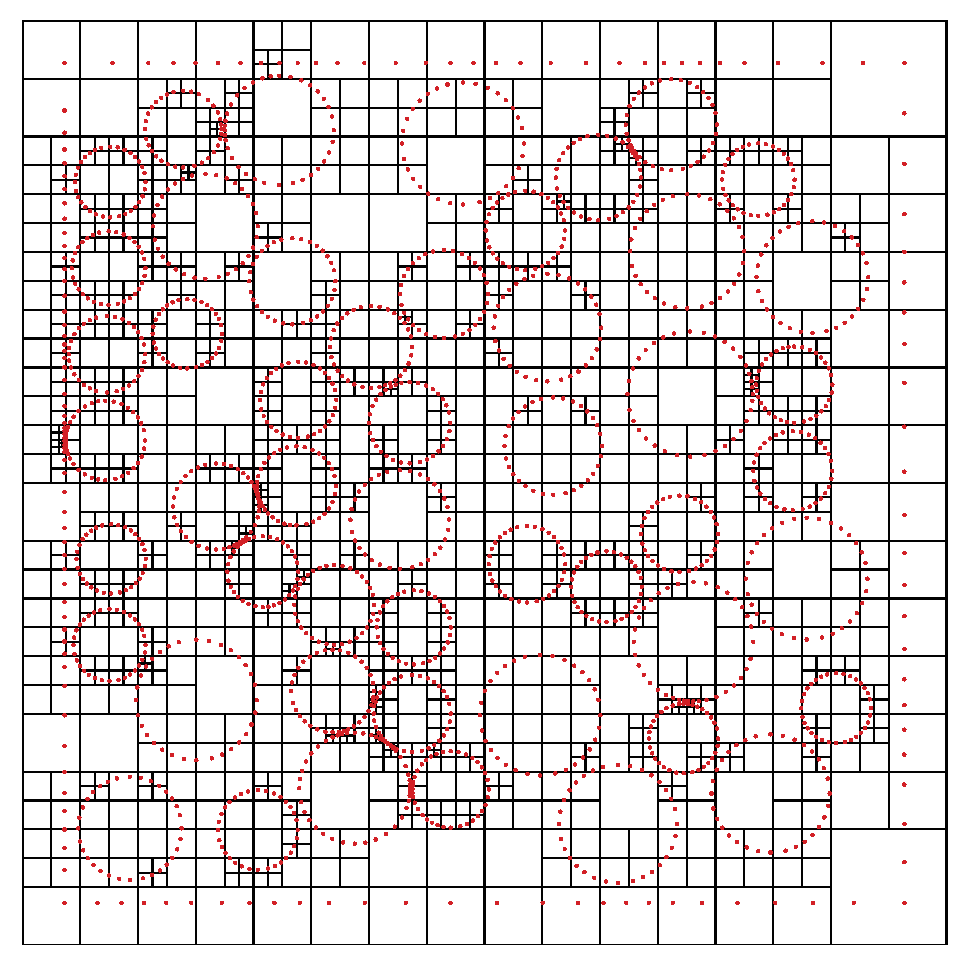
\includegraphics[width=0.8\textwidth]{pics/vf0.4686.eps}
	\end{center}
	\caption{孔隙率为0.4686的单胞自适应树结构}
	\label{fig:porous0_4686}
\end{figure}

\subsection{开孔材料三维几何建模}

可以借鉴的方法就是纤维复合材料的建模,把纤维拿掉不就是开孔材料了吗?

可以考虑的问题有孔洞的半径(大小),走向等几何因素对物理过程模拟的影响,
这些影响包括对物理模型的影响,数值计算模型中的网格的影响等等

现在我只有一个想法,纤维在单胞里面就可以看作是孔洞。纤维复合材料的建模就可以做为这样的模型,只要将纤维挖掉就可以了。这是第一个想法。
但是现在还有的问题就是考虑纤维(孔洞)的分布,走向的问题,不要让孔洞材料成为一个散乱的模型。
\newpage
\section{边界元方法一些内容简记}
参考内容主要为\cite{zhu1991,zhu2009},
\subsection{位势}
边界元方法关心的是如何用边界上的积分形式来表示所求的物理量,然后对边界积分方程离散化以后求解,
得到边界积分方程的途径是多样的,但是边界积分方程中包含的一些基本的组成部分,借用物理学中的概念
称其为\textbf{位势}。

常见的位势有
\begin{eqnarray}
	\text{对数位势} & u(y) & =  \frac{1}{2\pi}\int_{\color{red}{\Omega}}\rho(x)\ln\frac{1}{|{x-y}|}d\color{red}{x} \\
	\text{单层位势} & u(y) & =  \frac{1}{2\pi}\int_{\color{red}{\Gamma}}\sigma(x)\ln\frac{1}{|{x-y}|}d\color{red}{S_x} \\
	\text{双层位势} & u(y) & =  -\frac{1}{2\pi}\int_{\color{red}{\Gamma}}\mu(x)\frac{\partial}{\partial n_x}\ln\frac{1}{|{x-y}|}d\color{red}{S_x}
	\label{weishi}
\end{eqnarray}
上面几式中的$\rho(x),\sigma(x),\mu(x)$成为\textbf{密度函数}.
\subsection{边界积分方程分类}
由微分方程的边值问题得到边界积分方程的过程称为边界归化,根据不同的边界归化方法,可以得到不同的边界积分方程,
常见的边界积分方程有如下几类,
\begin{itemize}
	\item \textbf{直接边界积分方程}:如果边界上的密度函数是给定的或待定的直接物理量,相应的联系已知边界条件和未知边界条件
		的积分方程。
	\item \textbf{间接边界积分方程}:若边界密度函数不是直接物理量,联系已知边界条件和未知边界条件
		的积分方程。
	\item \textbf{虚边界积分方程}:基本解方法(?)
	\item \textbf{自然边界积分方程}:引用Green函数来进行边界归化,自然边界归化是指也称正则边界归化,他利用Green函数将偏微
		分方程的边值问题化为含有发散积分有限部分的边界积分方程。
\end{itemize}
\subsection{奇异积分的处理}
边界元方法常常有的一个缺点就是奇异积分,尤其是自然边界元方法,它采用的Green函数在边界上是奇异的,进行数值离散的时候需要
进行数值积分,常见的积分手段有解析方法进行积分,另外还可以进行数值积分。

\begin{itemize}
	\item \textbf{解析积分}: 由于边界元积分的区域是边界单元,经常使用的单元都是直边的,应此可以得到其解析积分。
	\item \textbf{数值积分}:
\end{itemize}

\section{边界元方法的一些参考书籍}
\cite{liu2009fast,beer2008boundary,schanz2007boundary,wolf2003scaled,kerget2007domain}
\section{边界热辐射与热传导耦合问题的适定性}
\subsection{问题的提法}
\subsubsection{稳态问题}\cite{tiihonen1997stefan,tiihonen1997nonlocal}:\\
\begin{equation}
	\begin{cases}
		- k \Delta T = f,                  &\text{in} \  \Omega, \\
		T = T_0, \qquad                    &\text{on} \  \Gamma,\\
		k \frac{\partial T}{\partial n} = -q, &\text{on} \  \Sigma.\\
	\end{cases}
	\label{eq:station}
\end{equation}
其中在边界上引入辐射作用,则边界上满足下列条件,
\begin{equation}
	k\frac{\partial T}{\partial n} + G(\sigma T^4) = 0, \text{on} \ \Sigma.
	\label{eqrad}
\end{equation}
式\eqref{eqrad}中$G$是一个算子,他是按如下方式定义的:
\begin{eqnarray}
	G(\sigma T^4) = (I-K)R=((I-K)(I-(I-E)K)^{-1}E)(\sigma T^4)), \\
	R = \varepsilon\sigma T^4 + (1-\varepsilon)K(R) = (I-(1-\varepsilon)K)^{-1}\varepsilon\sigma T^4, \\
	K(f)(s) = \int_{\Sigma}w(s,z)f(z)dz, \forall s \in \Sigma, \forall f \in L^{\infty}(\Sigma),
	\label{eqoperators}
\end{eqnarray}
其中$w(s,z)$表示角系数。

文献\cite{tiihonen1997stefan,tiihonen1997nonlocal}中给出了上述问题解的
存在唯一性。


\subsubsection{瞬态问题}
文献\cite{metzger1999existence}中给出了瞬态热辐射热传导耦合问题。
\begin{equation}
	\begin{cases}
		e_t - k \Delta T = f,                  &\text{in} \  \Omega, \\
		T = T_0, \qquad                    &\text{on} \  \Gamma,\\
		k \frac{\partial T}{\partial n} = -q, &\text{on} \  \Sigma.\\
		k \frac{\partial T}{\partial n} = (I-K)\lambda, &\text{on} \  \Sigma.\\
		T(\cdot,0)=T_0, & \text{on} \ \Omega. \\
		\lambda - (1-\varepsilon)K\lambda=\varepsilon\sigma T^4.
		
	\end{cases}
	\label{eq:timedepand}
\end{equation}
其中一些定义稳态情形的一样。

\subsubsection{其他讨论该问题解存在性的文章}
\cite{Qatanani2006149,Qatanani2004797,druet2009weak,klein2003transient}
\cite{qatanani2005error,qatanani2005analysis,druetnoncompactness,laitinen2002asymptotic}
\cite{Bermudeza201163,druet2010weak}

\begin{remark}
	 这些文献都是讨论稳态或者瞬态的采取Stefan–Boltzmann boundary condition的热传导问题的解的存在唯一性问题的文献,这些文献中没有讲数值方法的有效性,所以可以做的东西是数值方法,以及数值方法的应用,应用于求解实际问题。
\end{remark}

\section{椭圆孔洞材料建模}

这个工作主要是于艳师姐的工作,在她的工作基础上,我进行了代码的改造,做出了如下的事情:
\begin{itemize}
	\item 将师姐的代码进行了整理,然后添加几个统一的接口函数.
	\item 修改了椭圆颗粒的随机分布的特性,添加了长轴短轴转角正态分布的几何模型生成。
\end{itemize}
下面给出一些例子,分别用Python的matplotlib和asympote来画图,其中使用
asympote做的\figref{fig:asynormal}所示,并没有在\figref{fig:asynormal}
中添加边框,但是在画图的过程中可以添加标签,来标记椭圆。
\begin{figure}[htbp]
	\begin{center}
		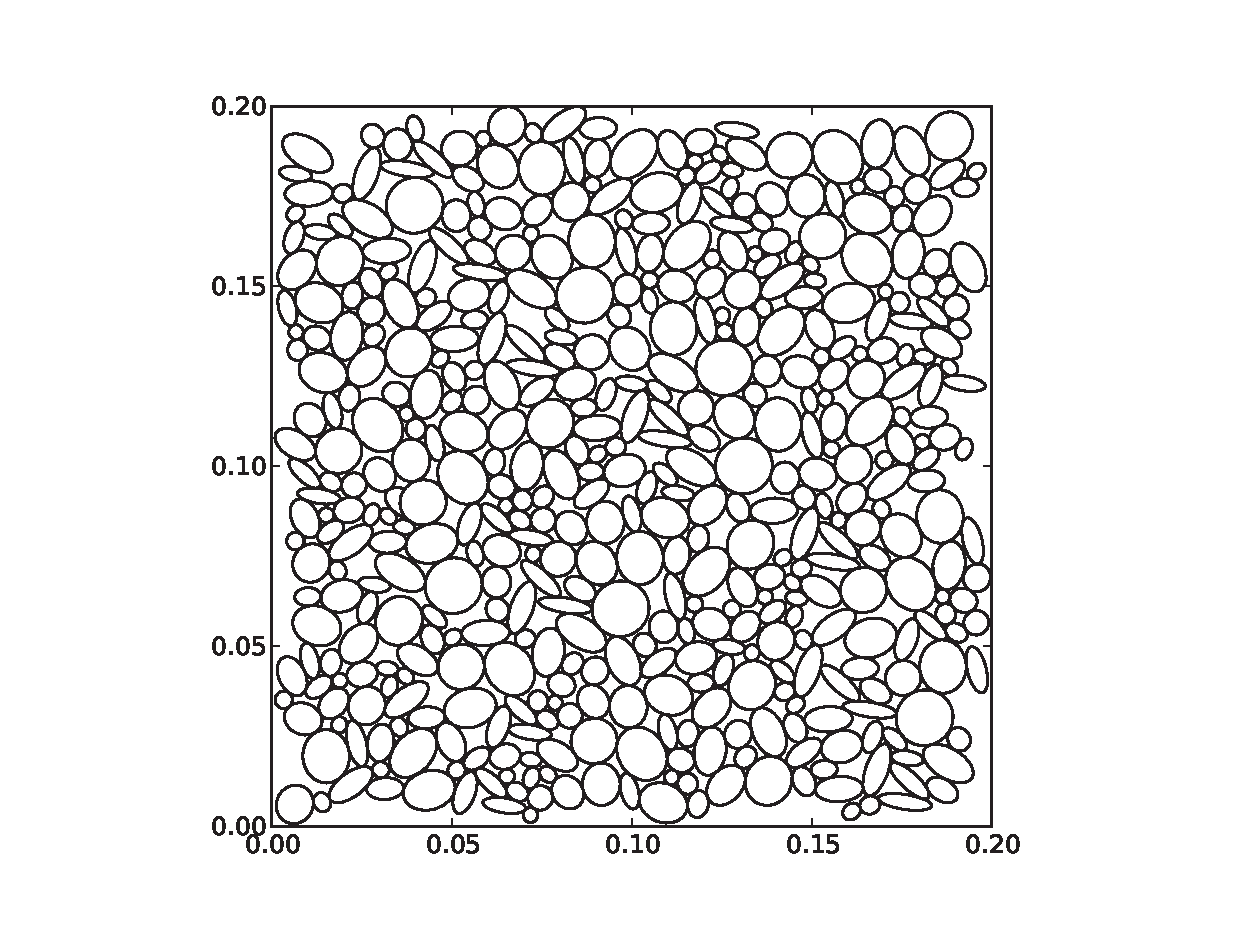
\includegraphics[width=0.8\textwidth]{pics/norm_destribution_1.eps}
	\end{center}
	\caption{紧凑的,与边界不相交,几何参数均匀分布的椭圆}
	\label{fig:normal1}
\end{figure}
\begin{figure}[htbp]
	\begin{center}
		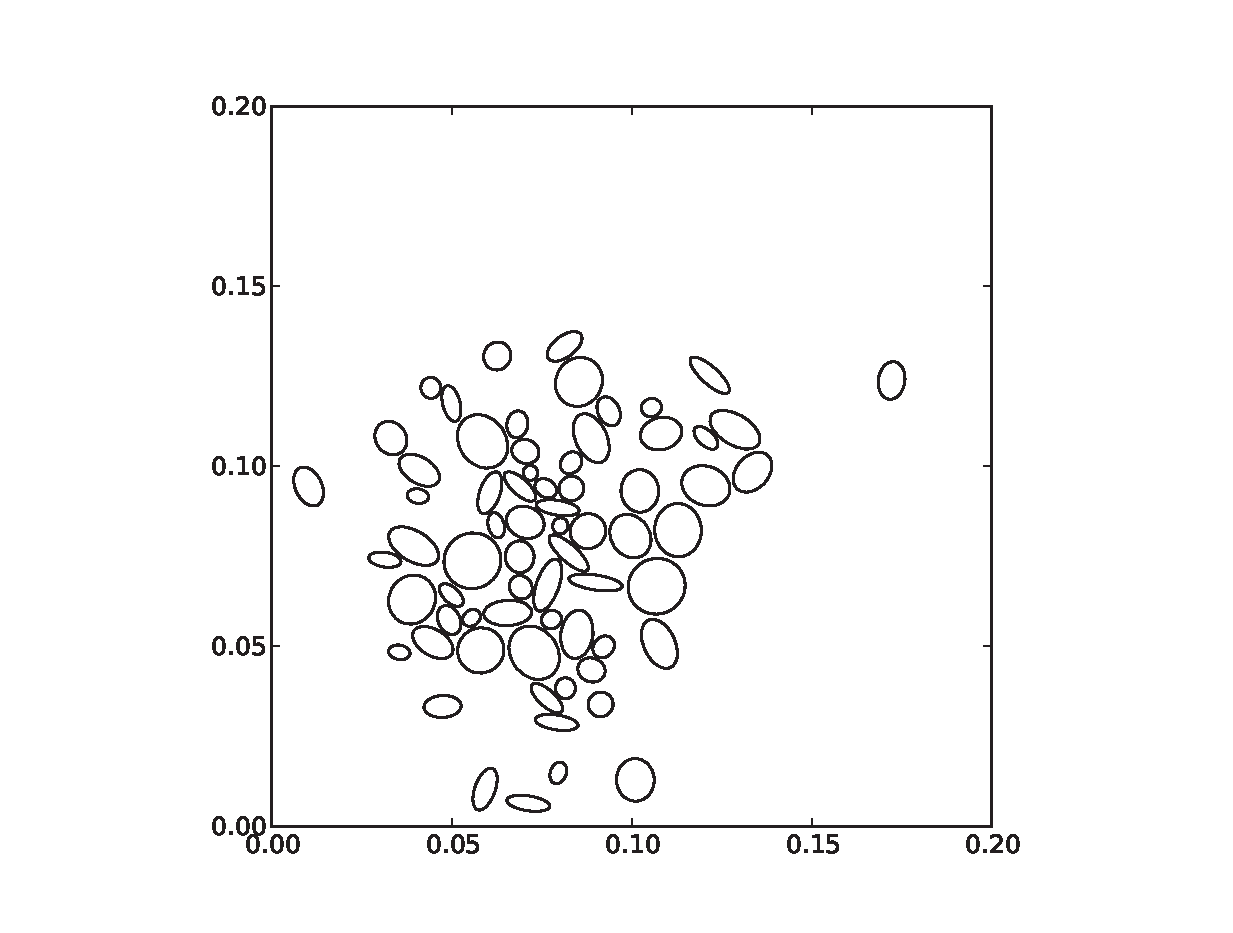
\includegraphics[width=0.4\textwidth]{pics/norm_destribution_2.eps}
		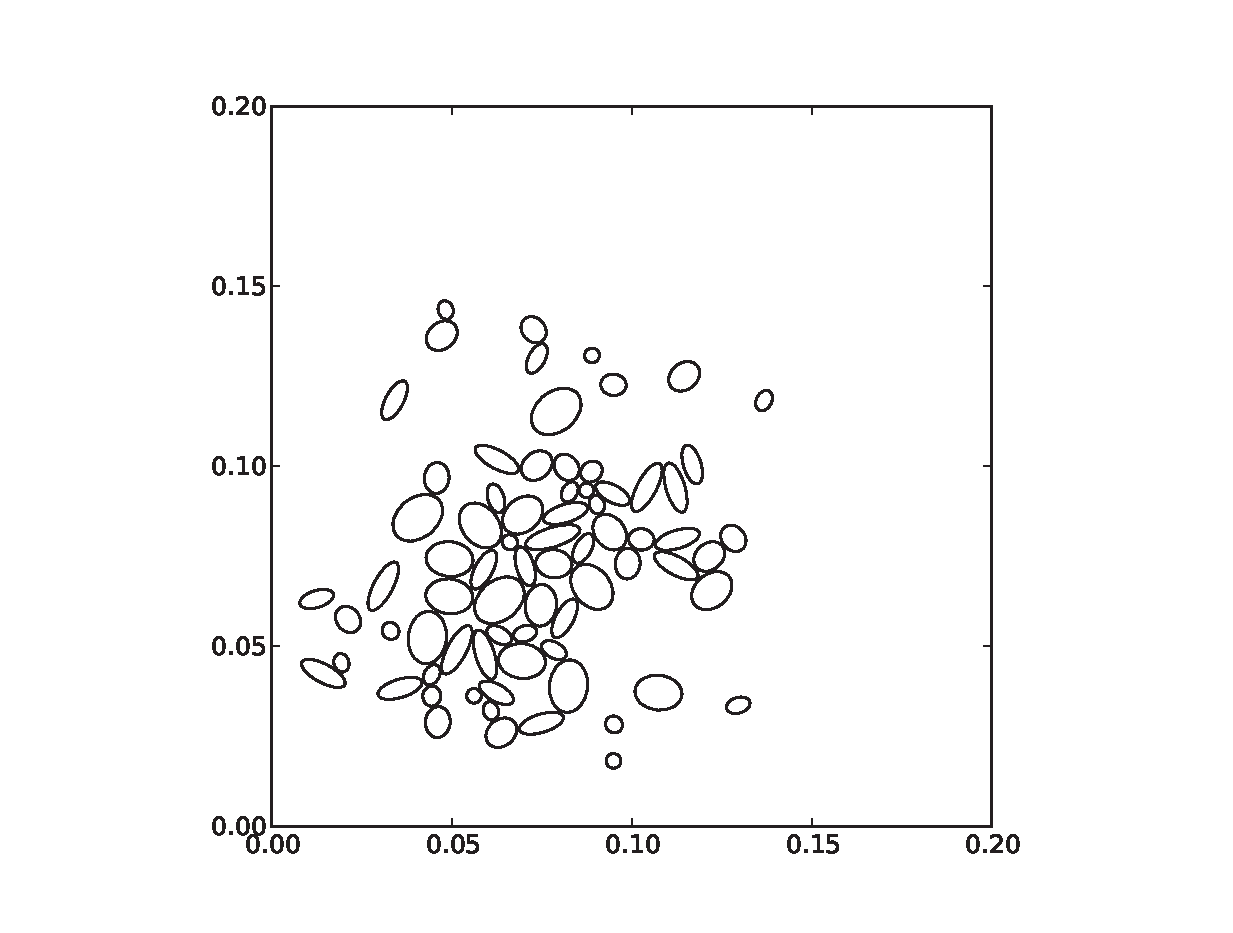
\includegraphics[width=0.4\textwidth]{pics/norm_destribution_3.eps}
	\end{center}
	\caption{舍选的两种位置正态分布的椭圆}
	\label{fig:normalshexuan}
\end{figure}
\begin{figure}[htbp]
	\begin{center}
		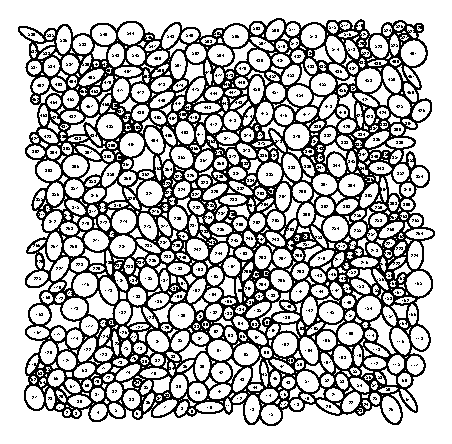
\includegraphics[width=0.5\textwidth]{pics/norm_destribution_1_asy.eps}
	\end{center}
	\caption{采用asy画的紧凑分布的椭圆}
	\label{fig:asynormal}
\end{figure}
\begin{figure}[htbp]
	\begin{center}
		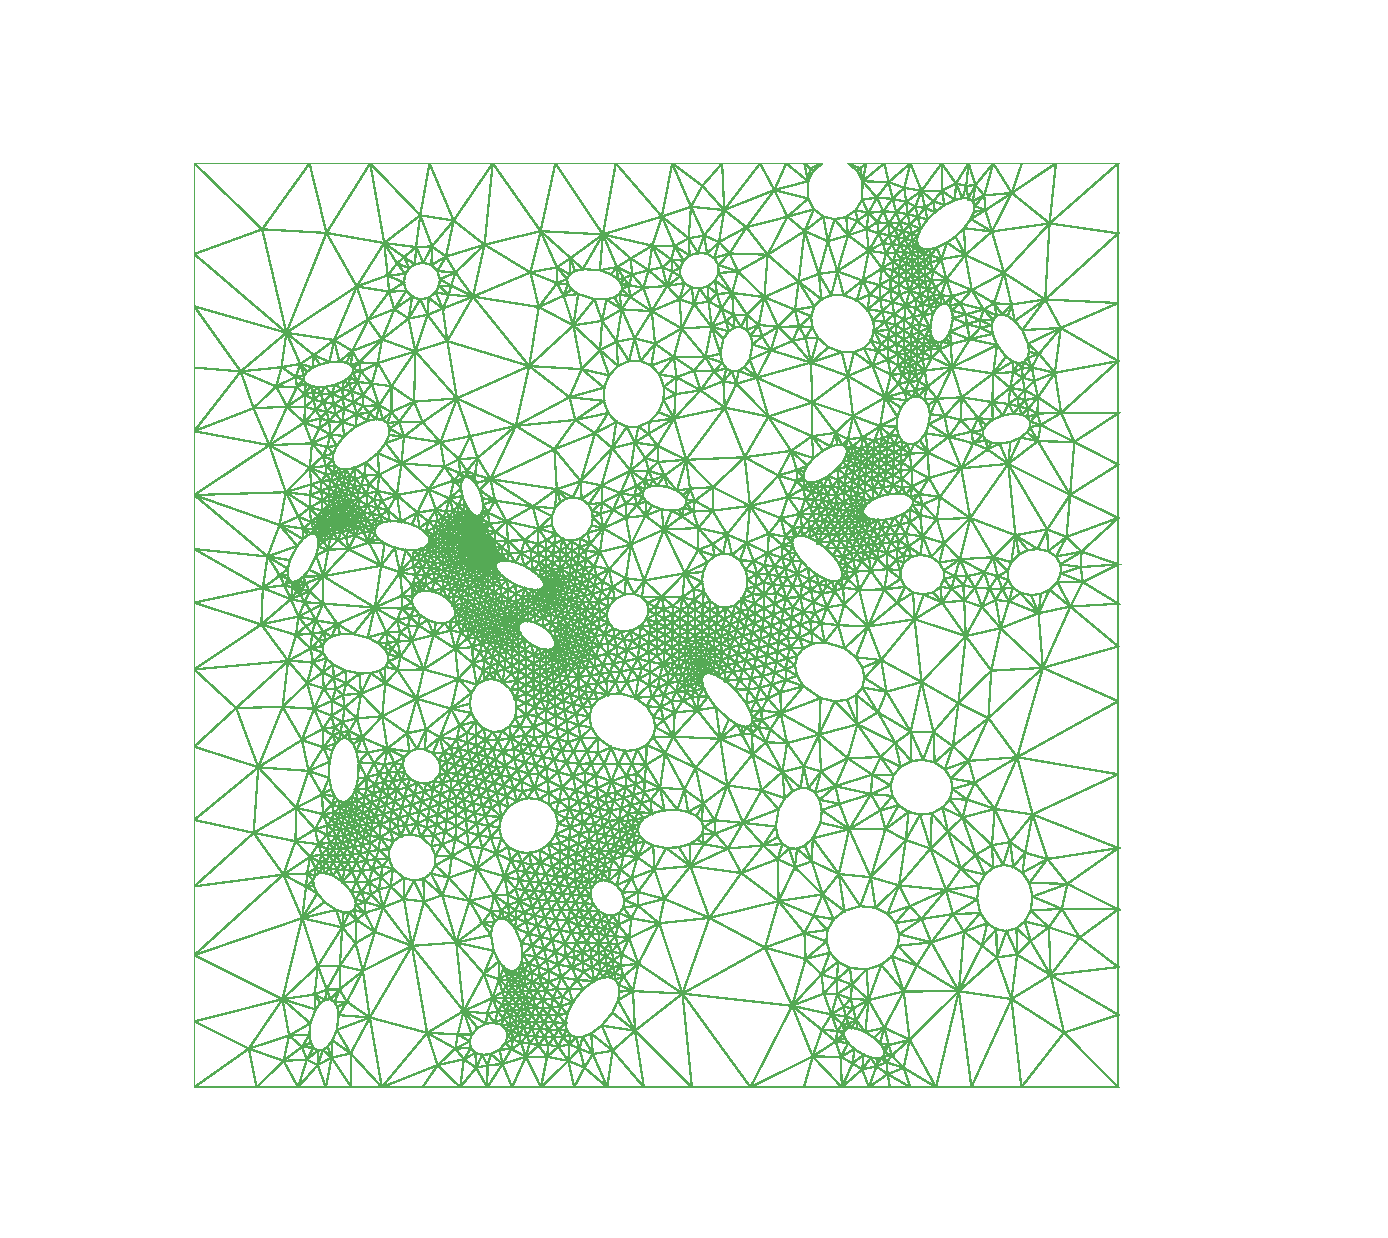
\includegraphics[width=0.8\textwidth]{pics/fem_ellipse_hole_mesh.eps}
	\end{center}
	\caption{孔洞材料网格剖分}
	\label{fig_ellipsemesh_hole}
\end{figure}
\begin{figure}[htbp]
	\begin{center}
		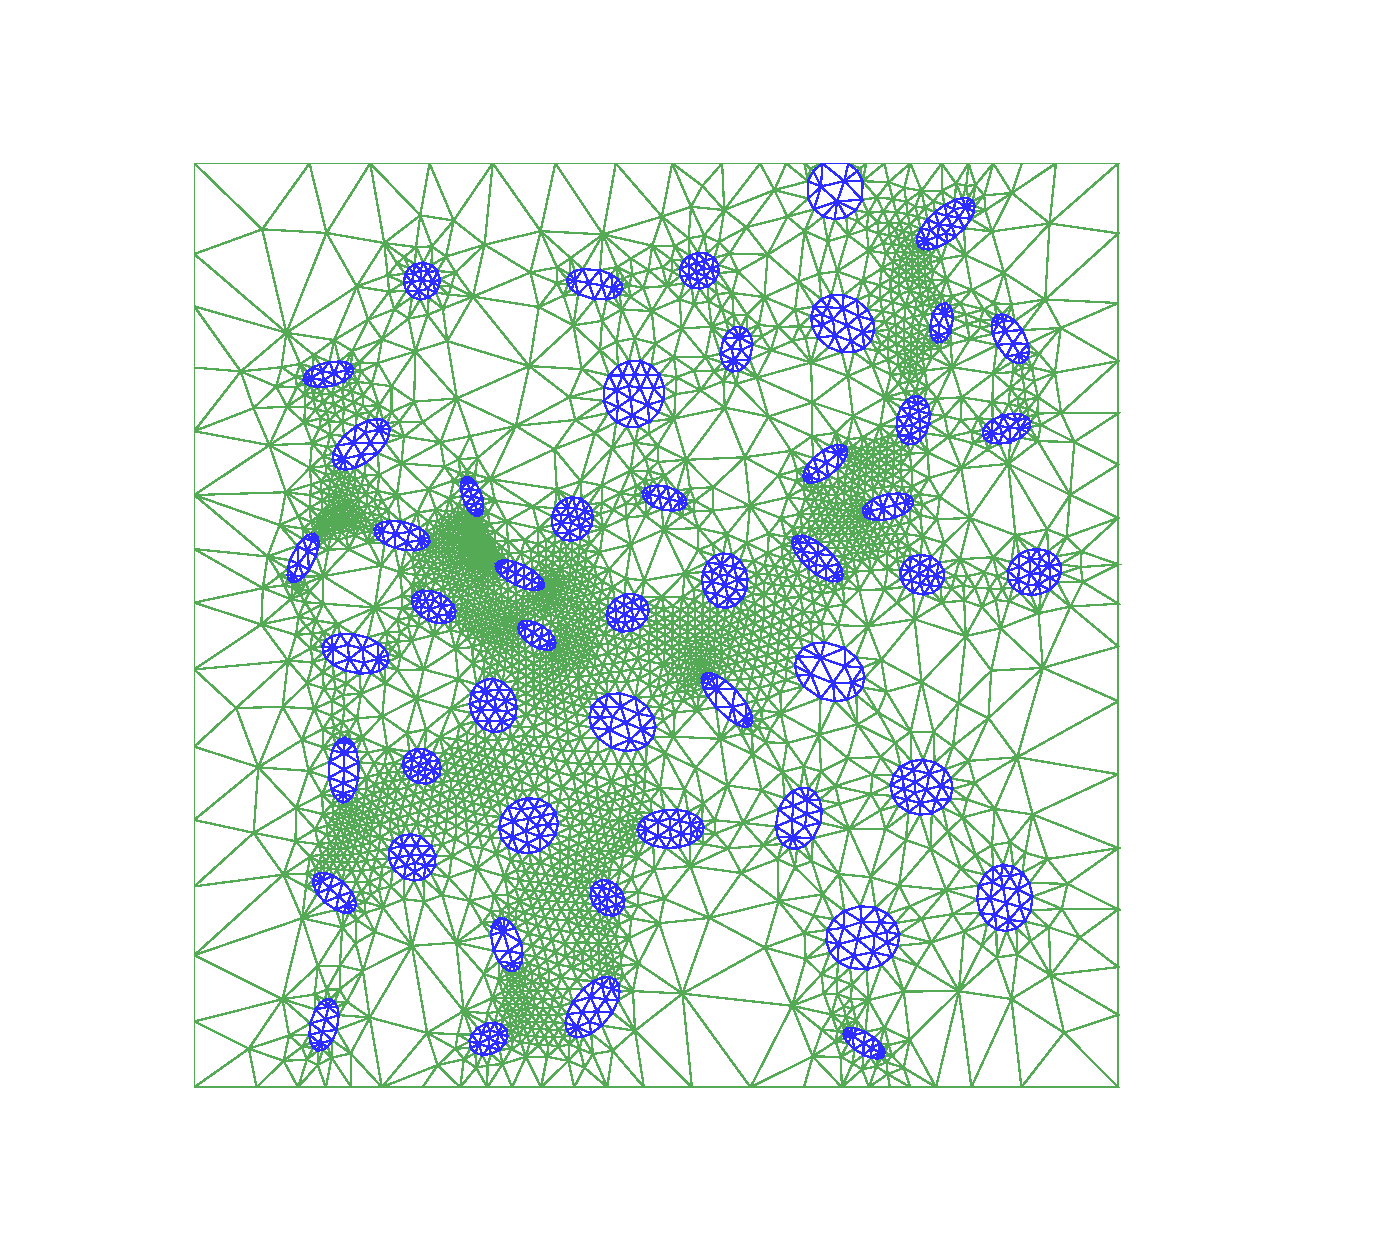
\includegraphics[width=0.8\textwidth]{pics/fem_ellipse_grain_mesh.eps}
	\end{center}
	\caption{颗粒增强材料网格剖分}
	\label{fig_ellipsemesh_grain}
\end{figure}

\section{二维孔隙率材料的边界元网格剖分}
基于前面一节的几何建模,可以构造出一个体分比很高的椭圆孔洞单胞模型,并且孔洞的几何参数什么
的都可以服从某种随机分布,在研究代表性单元时可以很好地利用。

\subsection{边界元网格需求}
在二维情形下,最基本的网格就是直线段,并且考虑到计算的过程中需要计算单元的法向导数,那么就要规定
单元的法向导数,在建模的过程中已经得到了椭圆的几何参数,根据参数方程就可以给出该模型的网格剖分。

对于每一个椭圆孔洞来说,规定单元走向都是顺时针,这样得到的单元的法向量都是指向孔洞内部,而不是区域内部。
\begin{figure}[h]
	\begin{center}
		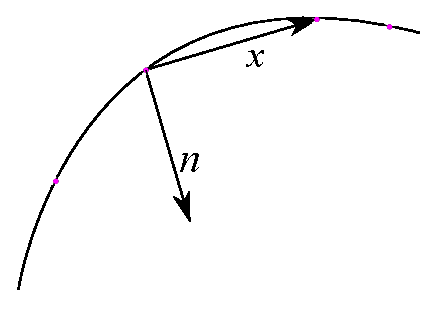
\includegraphics[width=0.4\textwidth]{pics/vec_right.eps}
		\caption{向量的右法向量}
	\end{center}
	\label{fig_vecright}
\end{figure}
在平面上一个向量的正交向量有两个,一个在向量的左边,一个在向量的右边。
\begin{definition}
	若向量$\mathbf{a}$与向量$\mathbf{b}$互相垂直并且向量积$\mathbf{a}\times\mathbf{b}$与垂直纸面的向量方向相同,那么称向量$\mathbf{a}$是向量$\mathbf{b}$的右法向量。
\end{definition}
\begin{lemma}
	若向量$\mathbf{b}$是向量$\mathbf{a}$的右法向量,则混合积$(\mathbf{a},\mathbf{b},\mathbf{a}\times\mathbf{b}) > 0 $.	
	\label{lem_vec_right}
\end{lemma}
\begin{lemma}
	向量$\mathbf{a}=(a_1,a_2)$的单位右法向量为$\frac{1}{\sqrt{a_1^2+a_2^2}}(-a_2,a_1)$.
	\label{lemma_vec_right}
\end{lemma}
\begin{figure}[h]
	\begin{center}
		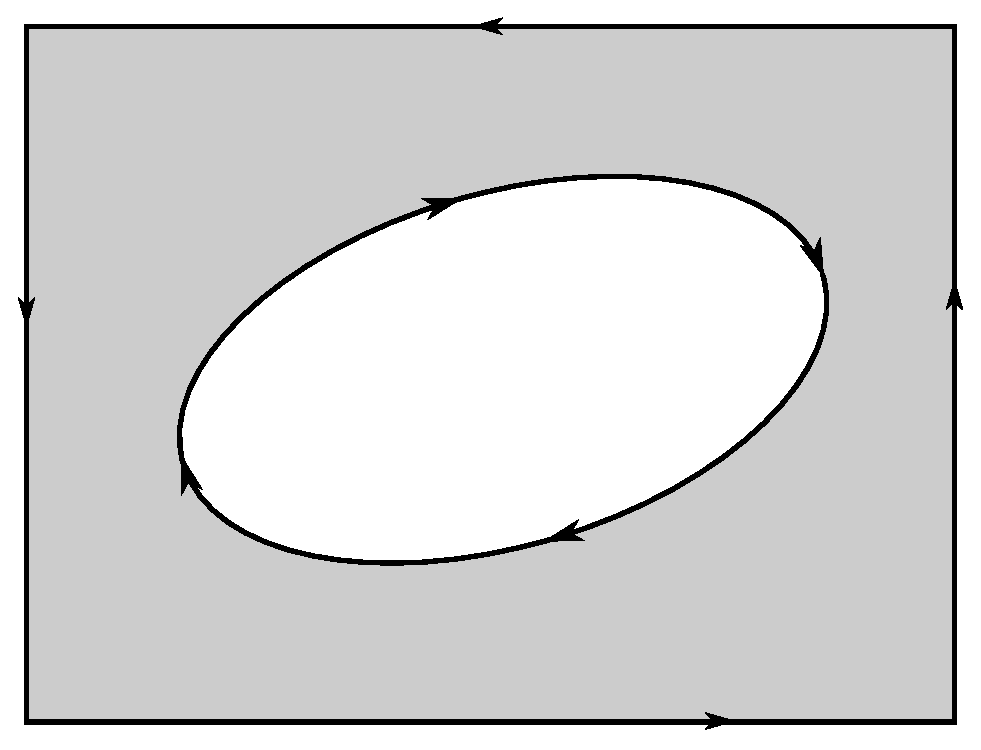
\includegraphics[width=0.4\textwidth]{pics/hole_towards.eps}
	\end{center}
	\caption{边界的方向}
	\label{fig_towards}
\end{figure}
\begin{figure}[h]
	\begin{center}
		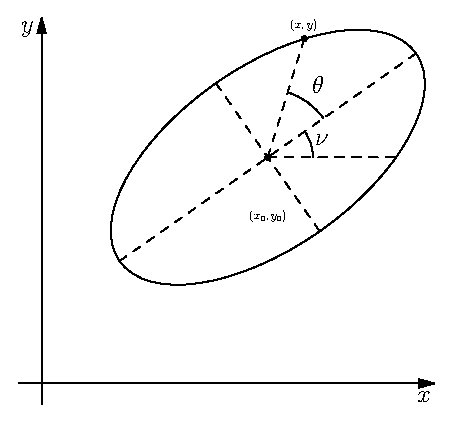
\includegraphics[width=0.4\textwidth]{pics/ellipse.eps}
	\end{center}
	\caption{椭圆的参数方程}
	\label{fig_ellipse_eq}
\end{figure}
\subsection{二维边界网格的生成}
下面对边界元网格的数据结构做出规定,
\begin{itemize}
	\item 单元节点信息,$node[i][j]$,$i$表示节点编号,$j$表示第$j$个坐标;
	\item 单元信息,$element[i][j]$,$i$表示单元编号,$j$表示第$j$个节点编号,节点编号满足:假设单元包含两个节点,节点1和节点2,若节点1指向节点2的向量的右法向量指向区域外,对于边界来说就是边界外,对于孔洞来说就是孔洞内部,那么在单元列表里面的节点顺序应该为1,2。
\end{itemize}

在上一节考虑的多孔材料中,椭圆的参数方程是
\[\left\{ {\begin{array}{*{20}{c}}
  {x - {x_{\text{0}}} = a\cos \theta \cos \nu  - b\sin \theta \sin \nu ,} \\ 
  {y - {y_{\text{0}}} = a\cos \theta \sin \nu  + b\sin \theta \cos \nu ,} 
\end{array}} \right.\]
其中$\theta$为参数,它表示椭圆中心到椭圆上一点组成的向量与椭圆长轴的夹角,它的范围为$[0,\pi]$。由\figref{fig_ellipse_eq}可以知道,只要顺时针取点就可以得到
相应的单元和节点,对应于椭圆孔洞,参数$\nu$的选取应该是从$\pi$到$0$选取,则可以得到满足其右法向量指向区域外部的要求。


\subsection{边界元程序中的边界条件的表示}
在热传导问题中,边界元方法要求解的未知变量通常是边界上的温度,或者是边界法向热流密度。
\subsubsection{数据结构}
两个数组$bctags[]$和$bcvalues[]$长度分别是边界上的自由度数,其中bctags是一个标记数组,
用来表示边界上是给定的是何种物理量,bcvalues表示的是该物理量在边界上的值。

ANSYS生成的边界元网格对于边界条件标记的是在单元标记,所以需要对单元文件读取,在对边界
自由度赋值。




\section{无矩阵边界元方法}

快速多极边界元方法的优点之一就是不需要显式的存储线性方程组的系数矩阵,而只需要借助于一定的手段来计算
一个迭代向量,也就是说进行一次矩阵向量乘法,实质上就是计算将迭代向量代入到积分中,计算了整个积分。因
此该方法是一种\textbf{无矩阵方法}。

对于传统的边界元也可以构造一种无矩阵的边界元方法,结合线性方程组的迭代算法,将迭代向量带入到边界积分
方程的积分的计算中去,采用线性方程组的迭代方法就可以构造一种无矩阵的边界元方法。下面以热传导方程的边
界积分方程为例来说明这种方法。

\section{四,八叉数结构的构造}

在快速多极边界元中,需要使用四,八叉数对单元的远近关系进行分组,因此需要对四八叉数中如何构造进行规定。

\begin{definition}
四叉树是一种树状的数据结构,每一个树节点有四个子节点。	
\end{definition}

二维快速多极边界元方法中的四叉树是指,将区域边界的正方形凸包逐次四分,直到
子节点中包含的单元数不超过给定的一个数。

\subsection{四叉树的数据结构}

现对快速多极边界元中使用的四叉树数据结构进行描述,
\begin{itemize}
	\item 用$l$表示树节点的编号;
	\item 数组$level[l]$表示第$l$个树节点的所在的层数;
	\item 数组$itree[l]$表示第$l$个树节点在相应层的坐标;
	\item 数组$ielem$是树结构中主要数据结构,他表示四叉树中每个节点包含的单元编号,他是一个$\textit{四叉树层数} \times \textit{边界元单元个数}$大小的数组;
	\item 数组$loct[l]$表示第$l$个树节点包含的单元在$ielem$中的索引;
	\item 数组$maxElem[l]$表示第$l$个树节点包含的单元个数;
	\item 数组$father[l]$表示第$l$个树节点的中心点;
	\item 数组$center[l]$表示第$l$个树节点的中心点;
	\item 数组$length[l]$表示第$l$个树节点的长度。 
\end{itemize}

四叉树的建立算法

树结构的最大深度估算

\begin{equation}
	depth_{max} = \log_4(\frac{(l_{min})^2}{4S_{root}}),
\end{equation}
其中$l_{min}$表示的是边界单元的最小边长,$S_{root}$表示的是根节点的面积。

生成四叉树的算法:
\begin{itemize}
	\item 计算一个方框把所有的节点包起来,并将该方框作为根结点;
	\item 令l = 1;遍历l-1层树节点,如果l-1层节点中单元数大于预设值,则将该节点一分为四,若l-1层节点中的单元数都小于预设值,则终止;
\end{itemize}



\section{快速多极算法中的一些概念}

快速多极算法建立在树结构上,利用树节点的远近关系来加速计算;

\begin{definition}
	邻接结点:与中心结点至少共有一个角点的树节点称为中心结点的邻接单元,如\figref{fignodetype}中淡蓝色所示; 
\end{definition}

\begin{definition}
	交互结点:若该树结点的父节点与中心结点的父节点互为邻接结点,并且不与中心结点的邻接,则称该节点为交互节点,如\figref{fignodetype}中黄色所示;
\end{definition}

\begin{definition}
	远程结点:既不是交互结点,也不是邻接结点的树结点,如\figref{fignodetype}中白色所示;
\end{definition}

快速多极算法中需要计算边界积分,每一次树遍历就是一次矩阵向量乘法,可以看作是做一次迭代向量的更新,
若把已知条件也就是边界条件也作为迭代向量的一部分,那么每次都要计算一次积分,不如将已知部分提取出来
作为迭代的右端向量,一次算好,以后都可以使用,可以节约计算时间。

\begin{figure}[htbp]
	\begin{center}
		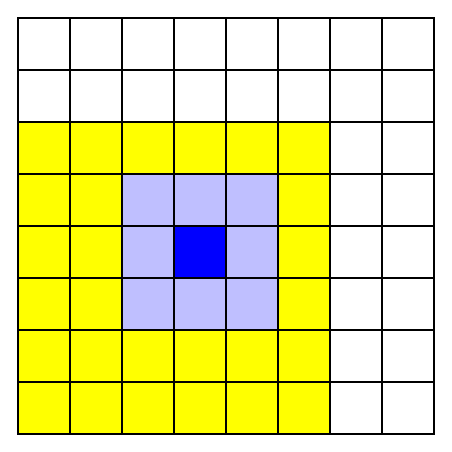
\includegraphics[width=0.4\textwidth]{pics/nabor.eps}
	\end{center}
	\caption{邻接结点,交互结点,远程结点}
	\label{fignodetype}
\end{figure}

\section{边界元积分策略}
\section{边界元线性系统求解的一般步骤}
\begin{itemize}
	\item 外层循环为单元循环,第一步是布置单元自由度,确定单元自由度局部编号到全局编号的映射关系
	\item 开始源点的循环,并生成源点,如果可能生成单位法向量,计算积分要使用;
	\item 求解单元矩阵,需要在单元上求积分,判断源点是否在单元上,若在则需要求解奇异积分,若非则使用gauss积分求解单元积分。
	\item 将生成的单元矩阵累加到系统矩阵中,同时施加边界条件,根据整体编号,判断边界上若温度已知则将热流密度之前的矩阵系数
		累加到左端矩阵中,并将温度矩阵之前的系数乘以已知值累加到右端项中,若热流密度已知则将温度矩阵系数累加到左端矩阵中,将
		热流矩阵乘以已知的热流值累加到右端项中。
	\item 求解线性系统
	\item 后处理,求特定地方的物理量。
\end{itemize}



\section{边界元中角点的处理}
\section{热辐射角系数的处理}
$\mathbf{x}$和$\mathbf{y}$是辐射表面上的两点,则三维情形下,两者之间的辐射核函数为
\begin{equation}
	F(\mathbf{x},\mathbf(y))=\frac{[(\mathbf{x}-\mathbf{y}) \cdot \mathbf{n}_x][(\mathbf{y}-\mathbf{x}) \cdot \mathbf{n}_y]}{\pi \|\mathbf{x}-\mathbf{y}\|^4}
	=\frac{1}{\pi} \frac{\partial}{\partial \mathbf{n}_x}(\ln (\|\mathbf{x}-\mathbf{y}\|)) \cdot \frac{\partial}{\partial \mathbf{n}_y}(\ln (\|\mathbf{x}-\mathbf{y}\|))
\end{equation}

二维情形的辐射核函数是
\begin{equation}
	F(\mathbf{x},\mathbf{y})=\frac{[(\mathbf{x}-\mathbf{y}) \cdot \mathbf{n}_x][(\mathbf{y}-\mathbf{x}) \cdot \mathbf{n}_y]}{2\|\mathbf{x}-\mathbf{y}\|^3}
\end{equation}
辐射核函数满足如下的性质:
\begin{itemize}
	\item $F(\mathbf{x},\mathbf{y}) \ge 0$
	\item $F(\mathbf{x},\mathbf{y})=F(\mathbf{y},\mathbf{x})$
	\item $\int_{\Sigma}F(\mathbf{x},\mathbf{y}) d \gamma(\mathbf{y}) = 1$
\end{itemize}

角系数的计算可以通过边界单元数值积分来计算,但是有一个问题就是这个积分是一个奇异积分需要对这个积分进行很好的估计;

由辐射核函数的归一性可以知道对于场点所在的单元的数值积分可以通过
\begin{equation}
	\int_{\Gamma_j}w(x,y) d\gamma(y) = 1 - \sum_{j=0,i \ne j}^N \int_{\Gamma_j}w(x,y) d\gamma(y);
\end{equation}
在非对角单元上的数值积分不是奇异积分,但是若单元是直边的时候角系数的积分
\begin{equation}
	\int_{\Gamma_i}w(x_i,y) d \gamma(y) = 0, x_i \in \Gamma_i , (\Gamma_i \text{是直线或直面}) 
\end{equation}
\newpage
%% list references if any.
\putbib[20131020oldnotes]
\newpage
	
